%Contains the blocking and MPI parts of the theory
\subsubsection{Importance sampling}
		We now want to make the code more efficient, so we replace the brute
		force Metropolis algorithm with a walk in coordinate space biased
		by the trial wave function, an approach based on the Fokker-Planck
		equation and the Langevin equation for generating a trajectory in
		coordinate space.

		For one particle or walker, a diffusion process characterized by a
		time-dependent probability density $P\left(x,t\right)$ in one dimension
		we have the Fokker-Planck equation
		\begin{align}
			\frac{\partial P}{\partial t}=D\frac{\partial}{\partial x}\left(\frac{\partial}{\partial x}-F\right)P\left(x,t\right),
		\end{align}
		where $F$ is a drift term and $D$ is the diffusion coefficient.

		The new positions in coordinate space are found using the Langevin
		equation with Euler's method. We go from the Langevin equation
		\begin{align}
			\frac{\partial x(t)}{\partial t}=DF(x(t))+\eta
		\end{align}
		where $\eta$ is a random variable. This gives us a new position
		\begin{align}
			y=x+DF(x)\Delta t+\xi\sqrt{\Delta t}.
		\end{align}
		Here $\xi$ is gaussian random variable and $\Delta t$ is a chosen
		time step. $D$ comes from the factor $1/2$ in the kinetic energy
		operator, and is therefore equal to $1/2$ in atomic units.

		The process of isotropic diffusion characterized by a time-dependent
		probability density $P\left(\mathbf{x},t\right)$ will, as an approximation,
		obey the Fokker-Planck equation
		\begin{align}
			\frac{\partial P}{\partial t}=\sum_{i}D\frac{\partial}{\partial\mathbf{x_{i}}}\left(\frac{\partial}{\partial\mathbf{x_{i}}}-\mathbf{F_{i}}\right)P(\mathbf{x},t),
		\end{align}
		where $\mathbf{F}_{i}$ is component number $i$ of the drift term
		caused by an external potential, and $D$ is the diffusion coefficient.
		We set the left hand side equal to zero and obtain the convergence
		to a stationary probability density
		\begin{align}
			\frac{\partial^{2}P}{\partial{\mathbf{x_{i}}^{2}}}=P\frac{\partial}{\partial{\mathbf{x_{i}}}}\mathbf{F_{i}}+\mathbf{F_{i}}\frac{\partial}{\partial{\mathbf{x_{i}}}}P.
		\end{align}


		Inserting the drift vector, $\mathbf{F}=g(\mathbf{x})\frac{\partial P}{\partial\mathbf{x}}$,
		we get
		\begin{align}
			\frac{\partial^{2}P}{\partial{\mathbf{x_{i}}^{2}}}=P\frac{\partial g}{\partial P}\left(\frac{\partial P}{\partial{\mathbf{x}_{i}}}\right)^{2}+Pg\frac{\partial^{2}P}{\partial{\mathbf{x}_{i}^{2}}}+g\left(\frac{\partial P}{\partial{\mathbf{x}_{i}}}\right)^{2}
		\end{align}
		To meet the condition of stationary density the left hand side has
		to be zero. This means that the terms containing first and second
		order derivatives has to cancel each other, which is only possible
		if $g=\frac{1}{P}$. This yields
		\begin{align}
			\mathbf{F}=2\frac{1}{\Psi_{T}}\nabla\Psi_{T},
		\end{align}
		known as the quantum force. This so-called force pushes the walker
		towards regions of configuration space where the trial wave function
		is large, thus increasing the efficiency of the simulation. This is
		a great improvement on the Metropolis algorithm where the walker has
		the same probability to move in every direction.

		From the Fokker-Planck equation we get a transition probability given
		by Green's function
		\begin{align}
			G(y,x,\Delta t)=\frac{1}{(4\pi D\Delta t)^{3N/2}}\exp\left(-\frac{(y-x-D\Delta tF(x))^{2}}{4D\Delta t}\right)
		\end{align}
		This means that the Metropolis algorithm
		\begin{align}
			A(y,x)=\mathrm{min}(1,q(y,x))),
		\end{align}
		where
		\begin{align}
			q(y,x)=\frac{|\Psi_{T}(y)|^{2}}{|\Psi_{T}(x)|^{2}},
		\end{align}
		is replaced by the Metropolis-Hastings algorithm,
		\begin{align}
			q(y,x)=\frac{G(x,y,\Delta t)|\Psi_{T}(y)|^{2}}{G(y,x,\Delta t)|\Psi_{T}(x)|^{2}}
		\end{align}


\subsection{Implementation of MPI}
		As the calculations now become increasingly complex and heavy we implement MPI to make use of multiple processors. Personal computers today usually have two, four or sometimes eight processors, which will give a fairly good speedup to our calculations. With bigger atoms or systems it is crucial to implement a way to distribute calculation to multiple processors.

		Implementing MPI in the Monte Carlo method is very easy. As we deal with statistical values we can easily split up the problem. Each process will run its own set of samples. The number of samples used by each process is simply $n/p$, where $n$ is the total number of samples we want to do, and $p$ is the number of processes. In the end all processors send their results to the master process, which sums up the values and takes the average over all processes.

	\subsection{Blocking}
	\label{sec:blocking}
		Blocking refers to a method to more accurately estimate the error of the values obtained by the VMC algorithm. It's actually a completely separate and independent process. The basic idea lies on the correlations between all the measurements. If these are important enough, they will produce an increase in the error that needs to be taken into account. The reason behind this is related to the effective amount of measurements, if there are correlations there will be measurements that will contain less information, so these won't be as valuable as the rest and it will be as if there are \textit{less} measurementes than we actually have. Obviously this is a problem, the usual identification of the error with $\sqrt{\frac{\sigma}{n}}$ will be overly optimistic and a correction is needed.

		\begin{align}
			f_d=\frac{1}{n-d}\sum_{k=1}^{n-d}{\left(x_k-\bar{x}_n\right)\left(x_{k+d}-\bar{x}_n\right)}
		\end{align}

		Where $f_d$ is the correlation between measurements separated by a distance of $d$. This can be used to give an actual form to the correction factor:\\

		\begin{align}
			\tau=1+2\sum_{d=1}^{n-1}{\frac{f_d}{var\left(x\right)}}
		\end{align}

		This is the autocorrelation time and it relates the error with the variance:\\

		\begin{align}
			err^2=\frac{\tau}{n}var\left(x\right)
		\end{align}

		And the inverse of the first factor is actually the number of effective measurements (that are actually useful since they contain information):\\

		\begin{align}
			n_{eff}=\frac{n}{\tau}
		\end{align}

		The expression that relates the standard deviation with this correlation time is thus:\\

		\begin{align}
			\sigma=\sqrt{\left(\frac{1+2\tau/\Delta t}{n}\left(\bar{x^2}-\bar{x}^2\right)\right)}
		\end{align}

		Where $\Delta t$ is the time between samples, and it's commonly smaller than $\tau$. The main problem is that to compute $\tau$ a lot of time is needed, and this is not feasible in most cases.\\

		The solution is to use blocking, and the algorithm to do this is actually quite simple. The total amount of measurements is divided into blocks (hence the name) of a certain size, and for each block the standard deviation is obtained. When the standard deviation stops increasing as the block size does, the correlations are irrelevant and the value for it is ready.\\

\textbf{NB!!!!!!!!!!!! NEEDS TO BE MOVED TO RESULTS PART}

		\begin{figure}
			\centering 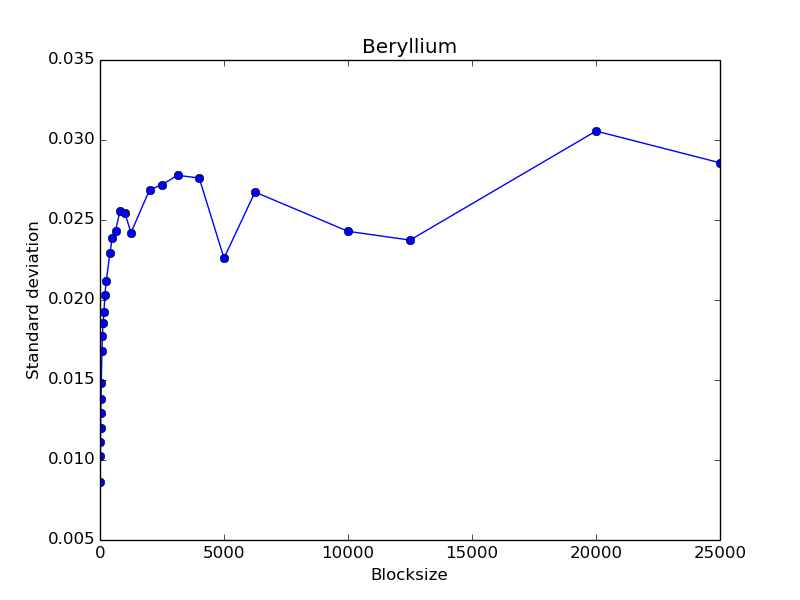
\includegraphics[width=0.45\linewidth]{../figures/Beryllium_blocking}
			\centering 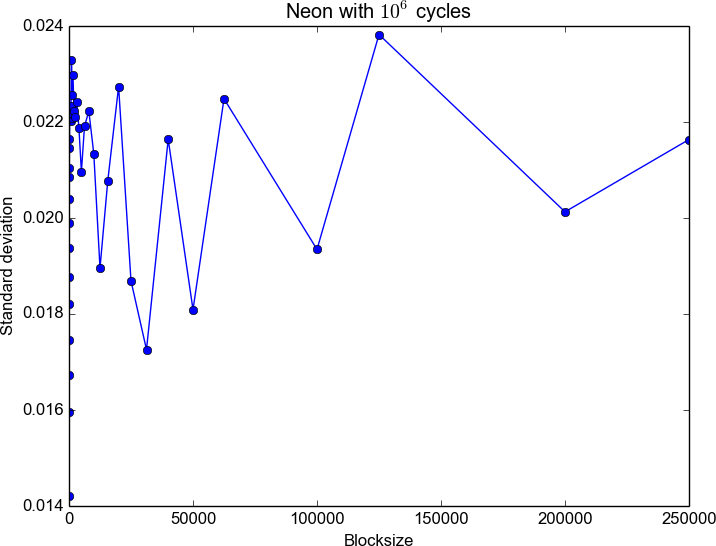
\includegraphics[width=0.45\linewidth]{../figures/Neon_blocking}
			\protect\caption{STD vs. blocksize with $10^{6}$ MC cycles.  The STD should have a plateauing trend as the blocksize increases.}\label{fig01:std_Stuff}
		\end{figure}


	\subsection{Energy minimization}
		As it can be expected, the values of the energy can depend heavily with respect to the variational parameters, so the optimal value must be found. This usually means finding the minimum value, and the first option would obviously be just a brute force search, but this is not efficient and there are better alternatives. Among these, we can find the steepest descent method, the conjugate gradient method and the Newton-Raphson method (also known as just Newton's method). The first two offer the posibility of finding a minimum in a multivariate space, while Newton's method only allows searching in one dimension, but is simpler and faster.\\

		Since these methods don't find minima but the zeros of a function, the derivative of said function is needed. But there is no analytical expression for the local energy, so a workaround must be used. It is possible to find an anlytical expression of this derivative as a function of the values of the local energy and the logarithmic derivative of the wave function. Following \parencite{mortens_notes} section $16.11$ the expression for the derivative with respect to parameter $c$ is:\\

		\begin{equation}\frac{\partial E}{\partial c}=2\left[\langle E_L\frac{\partial\ln{\Psi}}{\partial c}\rangle-E\langle\frac{\partial\ln{\Psi}}{\partial c}\rangle\right]\end{equation}

		Or more explicitly:\\

		\begin{equation}\frac{\partial E}{\partial c}=\frac{2}{N}\left[\sum_{i=1}^N\left(\left[E_L\left(c\right)\right]_i\left[\frac{\partial\ln{\Psi}}{\partial c}\right]_i\right)-\frac{1}{N}\sum_{i=1}^N\left(\left[E_L\left(c\right)\right]_i\sum_{i=1}^N\left[\frac{\partial\ln{\Psi}}{\partial c}\right]_i\right)\right]\end{equation}

		In our case, we are going to derive with respect to $\beta$ only, because we are only interested in minimization in that direction. Since the derivative is composed of three parts, two for the Slater determinants and one for the Padé-Jastrow interaction part, we get:\\

		\begin{equation}\frac{\partial\ln{\Psi}}{\partial\beta}=\frac{\partial\ln{\Psi_{SD\uparrow}}}{\partial\beta}+\frac{\partial\ln{\Psi_{SD\downarrow}}}{\partial\beta}+\frac{\partial\ln{\Psi_J}}{\partial\beta}=\frac{\partial\ln{\Psi_J}}{\partial\beta}\end{equation}
